%%A Presentation by Krishna Vaidyanathan

\documentclass[aspectratio=169]{beamer}

\usepackage{hyperref}
\usepackage{color}
\usepackage{multirow}
%\usepackage[font=tiny,labelfont=bf]{caption}[numbered]

%% Smart underlining -- from cdi-macros.tex
\def\ul#1{$\underline{\smash{\hbox{#1}}}$}

%% Shortcuts

\newcommand{\tabitem}{~~\llap{\textbullet}~~}

\newcommand{\bd}{\begin{description}}
\newcommand{\ed}{\end{description}}

\mode<presentation>
{
  \usetheme{Madrid}
  \useinnertheme{circles}
  \usecolortheme{beaver}
}
\usepackage[english]{babel}

\usepackage{times}
\usepackage[T1]{fontenc}
%
\title[Game-Theoretic Models]{Game-Theoretic Models of Information Overload in Social Networks}
\subtitle{A Presentation for CS886}
\author[Presented by Krishna Vaidyanathan]{Christian Borgs,\\Jennifer
    Chayes,\\Brian Karrer,\\Brendan Meeder,\\R. Ravi,\\Ray Reagans,\\Amin
    Sayedi\\\vspace{1em}Presented by Krishna Vaidyanathan}


\newcommand{\bi}{\begin{itemize}}
\newcommand{\ei}{\end{itemize}}

\newcommand{\bn}{\begin{enumerate}}
\newcommand{\en}{\end{enumerate}}

\begin{document}
\institute[UW]{University of Waterloo}
\frame[plain]{\titlepage}

\begin{frame}{Table of Contents}
\tableofcontents
\end{frame}

\section{Introduction}
\begin{frame}{Background}
    \bi
\item Increasing importance of social media.
    \pause
\item Some surveys claim the average person has five social media accounts and
    spends 1hr 40 mins on them every day \cite{telegraph15}.
    \pause
\item Increasing irrelevant updates on social media newsfeeds, or information overload.
    \ei
\end{frame}

\section{Types of Social Networks}
\subsection{Symmetric}
\subsection{Asymmetric}
\begin{frame}{Types of Social Networks}
    \bi
\item The paper considers two types of social media, namely:
    \pause
\item Symmetric: requires consent from both sides to maintain tie - eg.,
    Facebook.
    \pause
\item Asymmetric: requires consent from only one side to maintain tie - eg.,
    Twitter.
    \pause
\item Authors mainly look at asymmetric social networks.
    \ei
\end{frame}

\begin{frame}{Importance of information overload}
    \bi
\item Social networks make it convenient to get updates asynchronously.
    \pause
\item Makeup of newsfeed becomes very important to user.
    \pause
\item Mix of newsfeed is determined by the activity level of user's friends.
    \pause
\item \textit{How much one hears from one particular friend is not in user's 
        control.}
    \ei
\end{frame}

\section{Models for Social Networks}
\subsection{Followership}
\subsection{Engagement}
\begin{frame}{Models for Social Networks}
    \bi
\item  Assumptions of model:
    \pause
    \bi
\item Rate of sending updates is key decision variable.
    \pause
    \bi
\item Note that the paper shows empirical evidence to support this assumption.
    \ei
    \pause
\item Updates from friends are useful, but excessive updates have diminishing
    value.
    \pause
\item Users can be partitioned as producers and consumers of information (80 -
    20 rule).
    \ei
    \ei
\end{frame}

\begin{frame}{Models for Social Networks}
    \bi
\item Followership: Users in network will stay in network but unfollow agents
    who give too frequent updates.
    \pause
\item Engagement: Users get frustrated by high update rate of followees and
    leave the social network.
    \ei
\end{frame}

\begin{frame}{Graph Model}
    \bi
\item Complete bipartite graph on two disjoint sets of nodes: producers (C), and
    consumers (F).
    \pause
\item Edge between producer $i$ and consumer $j$ is associated with a non-negative
    quality score $q_{ij}$.
    \pause
    \bi
\item $q_{ij}$ denotes utility consumer $j$ derives from producer $i$'s updates.
    \ei
    \pause
\item Producer $i$ updates at a frequency (rate) of $r_{i}$.
    \pause
\item Payoff for producer $i$ is $r_i$ times the number of followers he/she has.
    \ei
\end{frame}

\section{Nash equilibrium}
\begin{frame}{Nash equilibrium}
    \bi
\item In Nash equilibrium, each player knows the strategy of other players, and
    no player has anything to gain by changing their strategy.
    \ei
\end{frame}

\section{Followership model}
\begin{frame}
    \begin{columns}[T]
        \begin{column}{0.2\textwidth}
            \begin{figure}[!ht]
                \centering
                \caption{Utility of Consumer for a Specific Producer}
                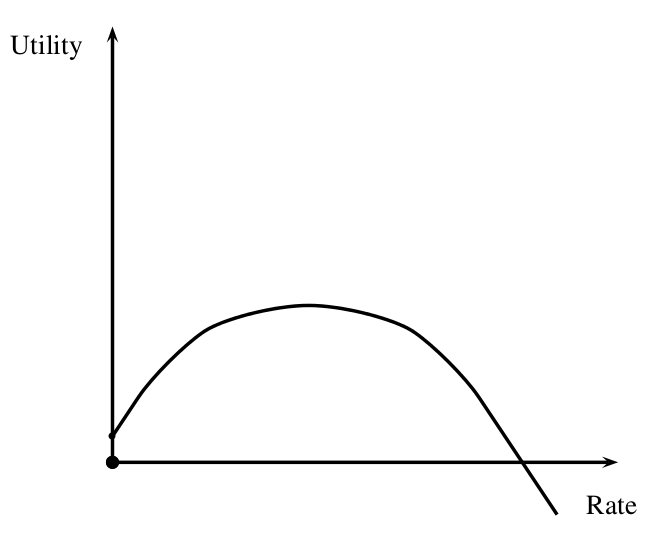
\includegraphics[scale=0.1]{./figures/follow_user_utility.png}
            \end{figure}
            \begin{figure}[!ht]
                \caption{Utility of a Producer}
                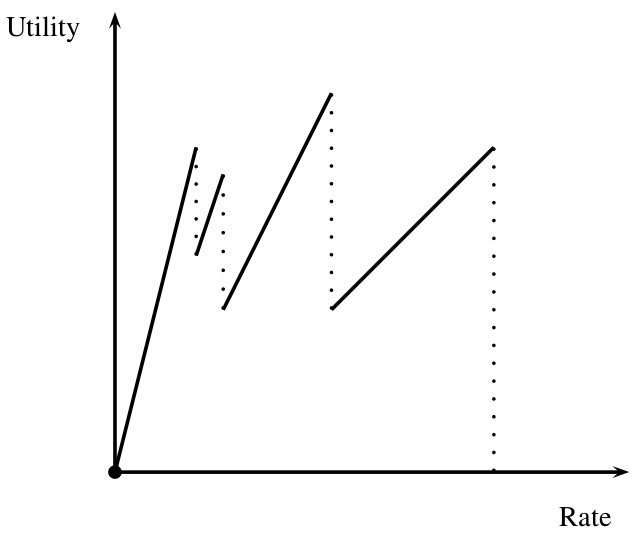
\includegraphics[scale=0.1]{./figures/follow_celeb_utility.png}
            \end{figure}
        \end{column}
        \begin{column}{0.4\textwidth}
            \pause
            \bi
        \item Utility for consumer $j$ is $U_{j} = r_{i}q_{ij} - \lambda (\sum_{i
                \in C_{j}}r_{i})^2$. $C_j$ being set of producers consumer $j$ follows.
            \pause
        \item Utility of consumer has an inverse U-shape, which was predicted by
            literature.
            \pause
        \item For producers, discontinuities at points where consumers stopped
            following.
            \ei
        \end{column}
    \end{columns}
\end{frame}

\begin{frame}{Fractional Following}
    \bi
\item First term of utility function represents benefit of consumer from tweets.
    \pause
\item Second term represents \textit{information overload} concept.
    \pause
\item For a consumer $j$, let $x_i$ represent the indicator variable of whether
    $j$ follows producer $i$ or not (1 if follows, 0 otherwise).
    \pause
\item $U_j = \sum_{i}x_i r_i q_{ij} - \lambda (\sum_{i}x_i r_i)$
    \pause
\item Very hard to solve if $x_i \in \{0, 1\}$, so simplify it to $x_i \in [0,1]$.
    \ei
\end{frame}

\begin{frame}{User strategy}
    \begin{block}{Proposition}
        Consider producer $i$ and fix the tweet-rate of the other producers. If
        $i$ increases his/her tweet-rate, his/her utility $U_i$ will not
        decrease.
    \end{block}
    \pause
    \bi
\item If producer $i$ increases her rate to $\alpha r_i$, consumer $j$ will
    correspondingly change $x_{ij}$ (at least $x_{ij}/\alpha$).
    \pause
\item If there exists a lower valued producer $l$, with $q_{il} < q_{ij}$,
    utility of $i$ strictly increases.
    \pause
\item Suggests that producers will tweet at a very high rate, and consumer will
    follow only one producer.
    \pause
\item Not very realistic...
    \ei
\end{frame}

\begin{frame}{Greedy Users}
    \bi
\item If consumer $j$ follows producer $i$ fractionally ($x_{ij} < 1$) then
    assume that consumer $j$ does not follow producer $i$ ($x_{ij} = 0$).
    \ei
    \pause
    \begin{block}{Definition}
        Consider consumer $j$ and let $q_1 \geq \ldots \geq q_n$ be the sorted
        order of $q_{1j},\ldots,q_{nj}$, and $k$ be the largest index such that
        $\sum_{i=1}^{k}r_i \leq q_k$. Under the greedy model, consumer $j$
        follows the $k$ producers for who he has the highest quality and no one
        else.
    \end{block}
\end{frame}

\begin{frame}{Example for Nash Equilibrium not existing}
    \begin{columns}[T]
        \begin{column}{0.2\textwidth}
            \begin{figure}
                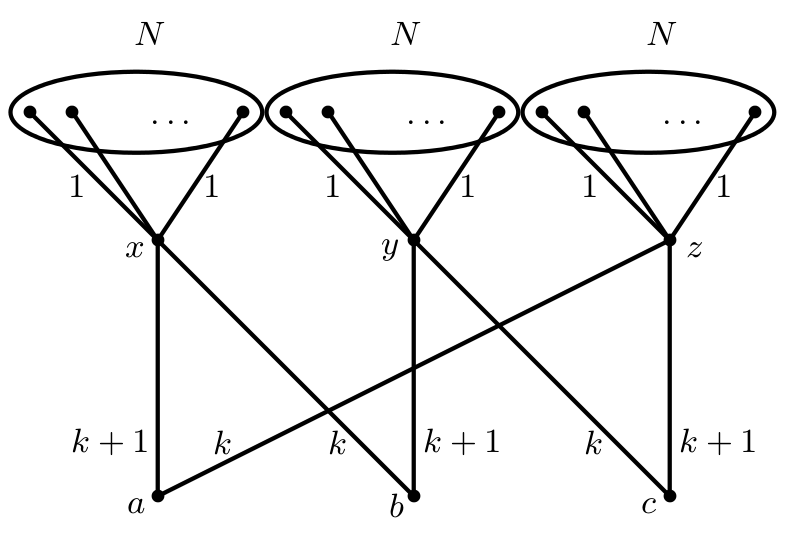
\includegraphics[scale=0.2]{./figures/follow_nash.png}
            \end{figure}
        \end{column}
        \begin{column}{0.2\textwidth}
            \pause
            \bi
        \item If $2k -2 > N > k + 1$, Figure does not have Nash equilibrium.
            \pause
        \item We do not prove this in slides...
            \ei
        \end{column}
    \end{columns}
\end{frame}

\begin{frame}{Examples of Nash Equilibrium existing}
    \bi
\item If all consumers follow the same global ranking of producers.
    \pause
    \bi
\item Note that if a producer $i$ changes his/her rate, utility of higher ranked producers
    is unchanged.
    \pause
\item Iteratively calculate equilibrium rate: $n$ steps for each producer.
    \pause
\item In step $i$, calculate optimum rate for producer $i$.
    \pause
\item Rate for higher ranked producers is the same as calculated in previous
    steps.
    \pause
\item Rate for lower ranked producers is set to 0 at step $i$.
    \ei
    \pause
\item Create a dependency graph for a game, where a directed edge is drawn between
    producers $x$ and $y$ if $q_{ix} > q_{iy}$.
    \pause
    \bi
\item If resultant graph is acyclic, Nash equilibrium exists.
    \pause
\item Similar argument as previously - nodes are topologically ordered and same
    induction argument.
    \ei
    \ei
\end{frame}

\begin{frame}{Matchings Characterizes Pure Rate Equilibrium}
    \bi
\item A consumer $i$ is said to be \textit{critical} to a producer $j$, if $j$
    drops $i$ if $r_i$ is increased.
    \pause
\item Find a matching from all subsets of producers to consumers that are
    critical for them.
    \pause
\item Check matching to see if it is a possible Nash equilibrium.
    \ei
\end{frame}

\section{Engagement Model}
\begin{frame}{Engagement Model - some notations}
    \bi
\item Let $F_i$ be the set of consumers that follow producer $i$.
    \pause
\item $C_j$ be the set of producers that consumer $i$ follows.
    \pause
\item Let $S$ be a function such that, $S(\sum_{i \in C_j}r_i)$ is the
    probability that consumer $j$ stays in the social network.
    \pause
\item Expected utility of producer $i$ is $U_{i}(r) = r_i(\sum_{j \in
        F_i}S(\sum_{i^{\prime}\in C_j}r_{i^{\prime}}))$.
    \ei
\end{frame}

\begin{frame}{Examples of Pure Nash equilibrium}
    \bi
\item When all consumers have same degree, or $|C_j| = d$ for all $j$.
    \pause
\item When all consumers follow one, or two producers.
    \pause
\item We do not prove this in the slides...
    \ei
\end{frame}

\section{Conclusions \& Thoughts}
\begin{frame}{Cons}
    \bi
\item In my opinion, not enough motivation as to why the particular models of social networks
    has been chosen.
\item Matching Characterization not elaborated upon, perhaps had to be
    shortened?
\item Understandable why fractional flow is considered in Followership model,
    but may not be realistic.
\item Could look at Mixed State Nash equilibrium?
    \ei
\end{frame}

\begin{frame}{Pros}
    \bi
\item Takes into account rate of information flow in social networks.
\item Characterizations of Nash equilibrium shown (in Followership model).
\item Empirical evidence to support rate of updates as a parameter.
    \ei
\end{frame}

\begin{frame}{References}
\begin{thebibliography}{9}
    \bibitem{borgs10}Borgs, C., Chayes, J., Karrer, B., Meeder, B., Ravi, R., Reagans,
    R., \& Sayedi, A. (2010). Game-theoretic models of information overload in
    social networks. In Algorithms and Models for the Web-Graph (pp. 146-161).
    Springer Berlin Heidelberg.
    \bibitem{telegraph15}
    \url{http://www.telegraph.co.uk/finance/newsbysector/mediatechnologyandtelecoms/11610959/Is-your-daily-social-media-usage-higher-than-average.html}
\end{thebibliography}

\end{frame}
\end{document}
